%!TEX program = xelatex

\documentclass[a4paper, openany, oneside]{memoir}
\usepackage[no-math]{fontspec}
\usepackage{pgfplots}
\pgfplotsset{compat=newest}
\usepackage{commath}
\usepackage{mathtools}
\usepackage{amssymb}
\usepackage{amsthm}
\usepackage{booktabs}
\usepackage{mathtools}
\usepackage{xcolor}
\usepackage[separate-uncertainty=true, per-mode=symbol]{siunitx}
\usepackage[noabbrev, capitalize]{cleveref}
\usepackage{listings}
\usepackage[american inductor, european resistor]{circuitikz}
\usepackage{amsmath}
\usepackage{amsfonts}
\usepackage{ifxetex}
\usepackage[dutch,english]{babel}
\usepackage[backend=bibtexu,texencoding=utf8,bibencoding=utf8,style=ieee,sortlocale=en_GB,language=auto]{biblatex}
\usepackage[strict,autostyle]{csquotes}
\usepackage{parskip}
\usepackage{import}
\usepackage{standalone}
\usepackage{hyperref}
%\usepackage[toc,title,titletoc]{appendix}

\ifxetex{} % Fonts laden in het geval dat je met Xetex compiled
    \usepackage{fontspec}
    \defaultfontfeatures{Ligatures=TeX} % To support LaTeX quoting style
    \setromanfont{Palatino Linotype} % Tover ergens in Font mapje in root.
    \setmonofont{Source Code Pro}
\else % Terug val in standaard pdflatex tool chain. Geen ondersteuning voor OTT fonts
    \usepackage[T1]{fontenc}
    \usepackage[utf8]{inputenc}
\fi
\newcommand{\references}[1]{\begin{flushright}{#1}\end{flushright}}
\renewcommand{\vec}[1]{\boldsymbol{\mathbf{#1}}}
\newcommand{\uvec}[1]{\boldsymbol{\hat{\vec{#1}}}}
\newcommand{\mat}[1]{\boldsymbol{\mathbf{#1}}}
\newcommand{\fasor}[1]{\boldsymbol{\tilde{\vec{#1}}}}
\newcommand{\cmplx}[0]{\mathrm{j}}
\renewcommand{\Re}[0]{\operatorname{Re}}
\newcommand{\Cov}{\operatorname{Cov}}
\newcommand{\Var}{\operatorname{Var}}
\newcommand{\proj}{\operatorname{proj}}
\newcommand{\Perp}{\operatorname{perp}}
\newcommand{\col}{\operatorname{col}}
\newcommand{\rect}{\operatorname{rect}}
\newcommand{\sinc}{\operatorname{sinc}}
\newcommand{\IT}{\operatorname{IT}}
\newcommand{\F}{\mathcal{F}}

\newtheorem{definition}{Definition}
\newtheorem{theorem}{Theorem}


\DeclareSIUnit{\voltampere}{VA} %apparent power
\DeclareSIUnit{\pii}{\ensuremath{\pi}}

\hypersetup{%setup hyperlinks
    colorlinks,
    citecolor=black,
    filecolor=black,
    linkcolor=black,
    urlcolor=black
}

% Example boxes
\usepackage{fancybox}
\usepackage{framed}
\usepackage{adjustbox}
\newenvironment{simpages}%
{\AtBeginEnvironment{itemize}{\parskip=0pt\parsep=0pt\partopsep=0pt}
\def\FrameCommand{\fboxsep=.5\FrameSep\shadowbox}\MakeFramed{\FrameRestore}}%
{\endMakeFramed}

% Impulse train
\DeclareFontFamily{U}{wncy}{}
\DeclareFontShape{U}{wncy}{m}{n}{<->wncyr10}{}
\DeclareSymbolFont{mcy}{U}{wncy}{m}{n}
\DeclareMathSymbol{\Sha}{\mathord}{mcy}{"58}
\addbibresource{../../../../includes/bibliography.bib}

\begin{document}

\section{Concept}
We will propose three different sampling methods
\begin{itemize}
\item circular sparse sampling
\item collaborative sampling
\item coprime sampling
\end{itemize}
Each of these techniques impose their own restrictions on sampling. Circular sparse ruler enforces that the sampling is done by a single device with multiple samplers with the same sample frequency. Collaborative sampling is done with multiple devices with multiple samplers with the same sample frequency. Coprime sampling enforces the use of one device with exactly two samplers, but allows for different sampling frequencies. Each sampling method is designed to perform well in situations where their restrictions are in order.

\subsection{Circular sparse sampling}
Circular sparse sampling uses samplers with each the same sampling period $NT$, where $T$ is the sampling period and $N$ the downsampling factor. Here $N$ refers to the downsampling factor discussed in \cref{sec:reconstruction-algorithm}. An example of circular sparse sampling where $N=7$ is illustrated in \cref{tkz:circsparseruler}.

\begin{figure}[H]
\centering
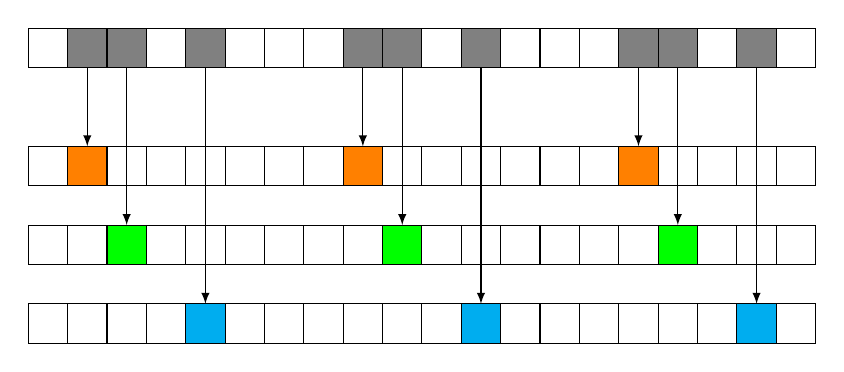
\begin{tikzpicture}
\draw  (-1,0.5) rectangle (-0.5,0);
\draw  [fill=gray](-0.5,0.5) rectangle (0,0);
\draw  [fill=gray](0,0.5) rectangle (0.5,0);
\draw  (0.5,0.5) rectangle (1,0);
\draw  [fill=gray](1,0.5) rectangle (1.5,0);
\draw  (1.5,0.5) rectangle (2,0);
\draw  (2,0.5) rectangle (2.5,0);
\draw  (2.5,0.5) rectangle (3,0);
\draw  [fill=gray](3,0.5) rectangle (3.5,0);
\draw  [fill=gray](3.5,0.5) rectangle (4,0);
\draw  (4,0.5) rectangle (4.5,0);
\draw  [fill=gray](4.5,0.5) rectangle (5,0);
\draw  (5,0.5) rectangle (5.5,0);
\draw  (5.5,0.5) rectangle (6,0);
\draw  (6,0.5) rectangle (6.5,0);
\draw  [fill=gray](6.5,0.5) rectangle (7,0);
\draw  [fill=gray](7,0.5) rectangle (7.5,0);
\draw  (7.5,0.5) rectangle (8,0);
\draw  [fill=gray](8,0.5) rectangle (8.5,0);
\draw  (8.5,0.5) rectangle (9,0);

\draw  (-1,-1) rectangle (-0.5,-1.5);
\draw  [fill=orange](-0.5,-1) rectangle (0,-1.5);
\draw  (0,-1) rectangle (0.5,-1.5);
\draw  (0.5,-1) rectangle (1,-1.5);
\draw  (1,-1) rectangle (1.5,-1.5);
\draw  (1.5,-1) rectangle (2,-1.5);
\draw  (2,-1) rectangle (2.5,-1.5);
\draw  (2.5,-1) rectangle (3,-1.5);
\draw  [fill=orange](3,-1) rectangle (3.5,-1.5);
\draw  (3.5,-1) rectangle (4,-1.5);
\draw  (4,-1) rectangle (4.5,-1.5);
\draw  (4.5,-1) rectangle (5,-1.5);
\draw  (5,-1) rectangle (5.5,-1.5);
\draw  (5.5,-1) rectangle (6,-1.5);
\draw  (6,-1) rectangle (6.5,-1.5);
\draw  [fill=orange](6.5,-1) rectangle (7,-1.5);
\draw  (7,-1) rectangle (7.5,-1.5);
\draw  (7.5,-1) rectangle (8,-1.5);
\draw  (8,-1) rectangle (8.5,-1.5);
\draw  (8.5,-1) rectangle (9,-1.5);

\draw  (-1,-2) rectangle (-0.5,-2.5);
\draw  (-0.5,-2) rectangle (0,-2.5);
\draw  [fill=green](0,-2) rectangle (0.5,-2.5);
\draw  (0.5,-2) rectangle (1,-2.5);
\draw  (1,-2) rectangle (1.5,-2.5);
\draw  (1.5,-2) rectangle (2,-2.5);
\draw  (2,-2) rectangle (2.5,-2.5);
\draw  (2.5,-2) rectangle (3,-2.5);
\draw  (3,-2) rectangle (3.5,-2.5);
\draw  [fill=green](3.5,-2) rectangle (4,-2.5);
\draw  (4,-2) rectangle (4.5,-2.5);
\draw  (4.5,-2) rectangle (5,-2.5);
\draw  (5,-2) rectangle (5.5,-2.5);
\draw  (5.5,-2) rectangle (6,-2.5);
\draw  (6,-2) rectangle (6.5,-2.5);
\draw  (6.5,-2) rectangle (7,-2.5);
\draw  [fill=green](7,-2) rectangle (7.5,-2.5);
\draw  (7.5,-2) rectangle (8,-2.5);
\draw  (8,-2) rectangle (8.5,-2.5);
\draw  (8.5,-2) rectangle (9,-2.5);

\draw  (-1,-3) rectangle (-0.5,-3.5);
\draw  (-0.5,-3) rectangle (0,-3.5);
\draw  (0,-3) rectangle (0.5,-3.5);
\draw  (0.5,-3) rectangle (1,-3.5);
\draw  [fill=cyan](1,-3) rectangle (1.5,-3.5);
\draw  (1.5,-3) rectangle (2,-3.5);
\draw  (2,-3) rectangle (2.5,-3.5);
\draw  (2.5,-3) rectangle (3,-3.5);
\draw  (3,-3) rectangle (3.5,-3.5);
\draw  (3.5,-3) rectangle (4,-3.5);
\draw  (4,-3) rectangle (4.5,-3.5);
\draw  [fill=cyan](4.5,-3) rectangle (5,-3.5);
\draw  (5,-3) rectangle (5.5,-3.5);
\draw  (5.5,-3) rectangle (6,-3.5);
\draw  (6,-3) rectangle (6.5,-3.5);
\draw  (6.5,-3) rectangle (7,-3.5);
\draw  (7,-3) rectangle (7.5,-3.5);
\draw  (7.5,-3) rectangle (8,-3.5);
\draw  [fill=cyan](8,-3) rectangle (8.5,-3.5);
\draw  (8.5,-3) rectangle (9,-3.5);

\draw [>=latex,->] (-.25,0) to (-.25,-1);
\draw [>=latex,->] (3.25,0) to (3.25,-1);
\draw [>=latex,->] (6.75,0) to (6.75,-1);

\draw [>=latex,->] (.25,0) to (.25,-2);
\draw [>=latex,->] (3.75,0) to (3.75,-2);
\draw [>=latex,->] (7.25,0) to (7.25,-2);

\draw [>=latex,->] (1.25,0) to (1.25,-3);
\draw [>=latex,->] (4.75,0) to (4.75,-3);
\draw [>=latex,->] (8.25,0) to (8.25,-3);

\end{tikzpicture}
\caption{An example of circular sparse ruler sampling with three samplers and $N=7$}\label{tkz:circsparseruler}
\end{figure}
The grey blocks represent the samples recovered by all samplers of the device. The coloured blocks represent the samples that are recovered by the different samplers. A possible implementation of this sampling method is illustrated in \cref{tkz:sc_circsparseruler}. 

\begin{figure}[H]
\centering
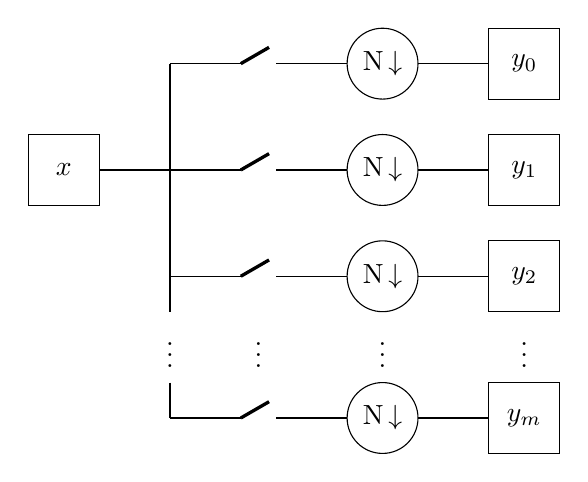
\begin{tikzpicture}[scale=.9]
\draw  (-2.5,2) rectangle (-1.5,1) node[pos=.5]{$x$};
\draw  (-1.5,1.5) -- (0.5,1.5);
\draw  (-0.5,3) -- (0.5,3);
\draw (-0.5,3) -- (-0.5,-0.5);

\node at (4.5,-1) {\vdots};
\node at (0.75,-1) {\vdots};
\node at (-0.5,-1) {\vdots};
\node at (2.5,-1) {\vdots};

\draw (-0.5,-1.5) -- (-0.5,-2);
\draw (-0.5,0) -- (0.5,0);
\draw (-0.5,-2) -- (0.5,-2);
\draw[ very thick](0.5,3)-- +(30:0.46);
\draw[ very thick](0.5,1.5)-- +(30:0.46);
\draw[ very thick](0.5,0)-- +(30:0.46);
\draw[ very thick](0.5,-2)-- +(30:0.46);

\draw  (1,3) -- (2,3);
\draw  (1,1.5) -- (2,1.5);
\draw  (1,0) -- (2,0);
\draw  (1,-2) -- (2,-2);

%\draw  (3,2) rectangle (2,1) node[pos=.5]{N$\,\downarrow$};
%\draw  (3,0.5) rectangle (2,-0.5) node[pos=.5]{N$\,\downarrow$};
%\draw  (3,-1.5) rectangle (2,-2.5) node[pos=.5]{N$\,\downarrow$};
%\draw  (3,3.5) rectangle (2,2.5) node[pos=.5]{N$\,\downarrow$};

\draw  (2.5,3) ellipse (.5 and .5) node{N$\,\downarrow$} ;
\draw  (2.5,1.5) ellipse (.5 and .5) node{N$\,\downarrow$} ;
\draw  (2.5,0) ellipse (.5 and .5) node{N$\,\downarrow$} ;
\draw  (2.5,-2) ellipse (.5 and .5) node{N$\,\downarrow$} ;

\draw  (3,3) -- (4,3);
\draw  (3,1.5) -- (4,1.5);
\draw  (3,0) -- (4,0);
\draw  (3,-2) -- (4,-2);

\draw  (5,2) rectangle (4,1) node[pos=.5]{$y_1$};
\draw  (5,0.5) rectangle (4,-0.5) node[pos=.5]{$y_2$};
\draw  (5,-1.5) rectangle (4,-2.5) node[pos=.5]{$y_m$};
\draw  (5,3.5) rectangle (4,2.5) node[pos=.5]{$y_0$};

\end{tikzpicture}
\caption{Schematic of a circular sparse ruler implementation}\label{tkz:sc_circsparseruler}
\end{figure}

The switches represent a sample and hold operation of the input signal $x$. The N$\,\downarrow$ represents an integrate and dump operation every $N$ samples. Therefore, $y_i$ is an $N$-decimation of the input signal. 

\subsection{Collaborative sampling}

Collaborative sampling is similar to circular sparse sampling, except for the fact that circular sparse sampling is restricted to only one device, while collaborative sampling is restricted to multiple devices. Collaborative sampling is illustrated in \cref{tkz:collaborative}. In this example, we use two devices with three samplers each and a downsampling factor of $N=13$.

\begin{figure}[H]
\centering
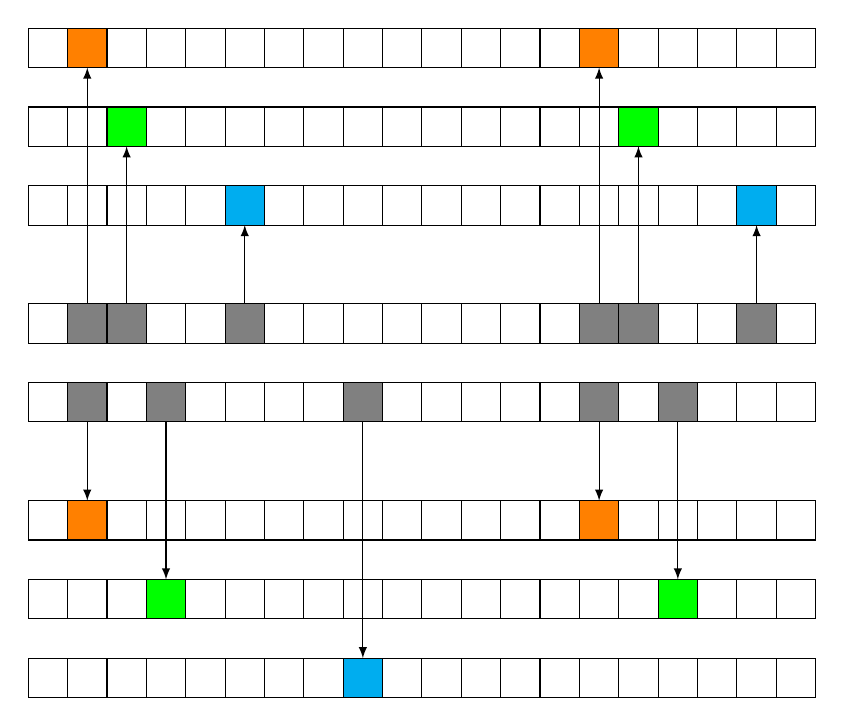
\begin{tikzpicture}
\draw  (-1,-4) rectangle (-0.5,-4.5);
\draw  [fill=gray](-0.5,-4) rectangle (0,-4.5);
\draw  [fill=gray](0,-4) rectangle (0.5,-4.5);
\draw  (0.5,-4) rectangle (1,-4.5);
\draw  (1,-4) rectangle (1.5,-4.5);
\draw  [fill=gray](1.5,-4) rectangle (2,-4.5);
\draw  (2,-4) rectangle (2.5,-4.5);
\draw  (2.5,-4) rectangle (3,-4.5);
\draw  (3,-4) rectangle (3.5,-4.5);
\draw  (3.5,-4) rectangle (4,-4.5);
\draw  (4,-4) rectangle (4.5,-4.5);
\draw  (4.5,-4) rectangle (5,-4.5);
\draw  (5,-4) rectangle (5.5,-4.5);
\draw  (5.5,-4) rectangle (6,-4.5);
\draw  [fill=gray](6,-4) rectangle (6.5,-4.5);
\draw  [fill=gray](6.5,-4) rectangle (7,-4.5);
\draw  (7,-4) rectangle (7.5,-4.5);
\draw  (7.5,-4) rectangle (8,-4.5);
\draw  [fill=gray](8,-4) rectangle (8.5,-4.5);
\draw  (8.5,-4) rectangle (9,-4.5);

\draw  (-1,-0.5) rectangle (-0.5,-1);
\draw  [fill=orange](-0.5,-0.5) rectangle (0,-1);
\draw  (0,-0.5) rectangle (0.5,-1);
\draw  (0.5,-0.5) rectangle (1,-1);
\draw  (1,-0.5) rectangle (1.5,-1);
\draw  (1.5,-0.5) rectangle (2,-1);
\draw  (2,-0.5) rectangle (2.5,-1);
\draw  (2.5,-0.5) rectangle (3,-1);
\draw  (3,-0.5) rectangle (3.5,-1);
\draw  (3.5,-0.5) rectangle (4,-1);
\draw  (4,-0.5) rectangle (4.5,-1);
\draw  (4.5,-0.5) rectangle (5,-1);
\draw  (5,-0.5) rectangle (5.5,-1);
\draw  (5.5,-0.5) rectangle (6,-1);
\draw  [fill=orange](6,-0.5) rectangle (6.5,-1);
\draw  (6.5,-0.5) rectangle (7,-1);
\draw  (7,-0.5) rectangle (7.5,-1);
\draw  (7.5,-0.5) rectangle (8,-1);
\draw  (8,-0.5) rectangle (8.5,-1);
\draw  (8.5,-0.5) rectangle (9,-1);

\draw  (-1,-1.5) rectangle (-0.5,-2);
\draw  (-0.5,-1.5) rectangle (0,-2);
\draw  [fill=green](0,-1.5) rectangle (0.5,-2);
\draw  (0.5,-1.5) rectangle (1,-2);
\draw  (1,-1.5) rectangle (1.5,-2);
\draw  (1.5,-1.5) rectangle (2,-2);
\draw  (2,-1.5) rectangle (2.5,-2);
\draw  (2.5,-1.5) rectangle (3,-2);
\draw  (3,-1.5) rectangle (3.5,-2);
\draw  (3.5,-1.5) rectangle (4,-2);
\draw  (4,-1.5) rectangle (4.5,-2);
\draw  (4.5,-1.5) rectangle (5,-2);
\draw  (5,-1.5) rectangle (5.5,-2);
\draw  (5.5,-1.5) rectangle (6,-2);
\draw  (6,-1.5) rectangle (6.5,-2);
\draw  [fill=green](6.5,-1.5) rectangle (7,-2);
\draw  (7,-1.5) rectangle (7.5,-2);
\draw  (7.5,-1.5) rectangle (8,-2);
\draw  (8,-1.5) rectangle (8.5,-2);
\draw  (8.5,-1.5) rectangle (9,-2);

\draw  (-1,-2.5) rectangle (-0.5,-3);
\draw  (-0.5,-2.5) rectangle (0,-3);
\draw  (0,-2.5) rectangle (0.5,-3);
\draw  (0.5,-2.5) rectangle (1,-3);
\draw  (1,-2.5) rectangle (1.5,-3);
\draw  [fill=cyan](1.5,-2.5) rectangle (2,-3);
\draw  (2,-2.5) rectangle (2.5,-3);
\draw  (2.5,-2.5) rectangle (3,-3);
\draw  (3,-2.5) rectangle (3.5,-3);
\draw  (3.5,-2.5) rectangle (4,-3);
\draw  (4,-2.5) rectangle (4.5,-3);
\draw  (4.5,-2.5) rectangle (5,-3);
\draw  (5,-2.5) rectangle (5.5,-3);
\draw  (5.5,-2.5) rectangle (6,-3);
\draw  (6,-2.5) rectangle (6.5,-3);
\draw  (6.5,-2.5) rectangle (7,-3);
\draw  (7,-2.5) rectangle (7.5,-3);
\draw  (7.5,-2.5) rectangle (8,-3);
\draw  [fill=cyan](8,-2.5) rectangle (8.5,-3);
\draw  (8.5,-2.5) rectangle (9,-3);

\draw [>=latex,->] (-0.25,-4) to (-0.25,-1);
\draw [>=latex,->] (6.25,-4) to (6.25,-1);

\draw [>=latex,->] (0.25,-4) to (0.25,-2);
\draw [>=latex,->] (6.75,-4) to (6.75,-2);

\draw [>=latex,->] (1.75,-4) to (1.75,-3);
\draw [>=latex,->] (8.25,-4) to (8.25,-3);

\draw  (-1,-5) rectangle (-0.5,-5.5);
\draw  [fill=gray](-0.5,-5) rectangle (0,-5.5);
\draw  (0,-5) rectangle (0.5,-5.5);
\draw  [fill=gray](0.5,-5) rectangle (1,-5.5);
\draw  (1,-5) rectangle (1.5,-5.5);
\draw  (1.5,-5) rectangle (2,-5.5);
\draw  (2,-5) rectangle (2.5,-5.5);
\draw  (2.5,-5) rectangle (3,-5.5);
\draw  [fill=gray](3,-5) rectangle (3.5,-5.5);
\draw  (3.5,-5) rectangle (4,-5.5);
\draw  (4,-5) rectangle (4.5,-5.5);
\draw  (4.5,-5) rectangle (5,-5.5);
\draw  (5,-5) rectangle (5.5,-5.5);
\draw  (5.5,-5) rectangle (6,-5.5);
\draw  [fill=gray](6,-5) rectangle (6.5,-5.5);
\draw  (6.5,-5) rectangle (7,-5.5);
\draw  [fill=gray](7,-5) rectangle (7.5,-5.5);
\draw  (7.5,-5) rectangle (8,-5.5);
\draw  (8,-5) rectangle (8.5,-5.5);
\draw  (8.5,-5) rectangle (9,-5.5);

\draw  (-1,-6.5) rectangle (-0.5,-7);
\draw  [fill=orange](-0.5,-6.5) rectangle (0,-7);
\draw  (0,-6.5) rectangle (0.5,-7);
\draw  (0.5,-6.5) rectangle (1,-7);
\draw  (1,-6.5) rectangle (1.5,-7);
\draw  (1.5,-6.5) rectangle (2,-7);
\draw  (2,-6.5) rectangle (2.5,-7);
\draw  (2.5,-6.5) rectangle (3,-7);
\draw  (3,-6.5) rectangle (3.5,-7);
\draw  (3.5,-6.5) rectangle (4,-7);
\draw  (4,-6.5) rectangle (4.5,-7);
\draw  (4.5,-6.5) rectangle (5,-7);
\draw  (5,-6.5) rectangle (5.5,-7);
\draw  (5.5,-6.5) rectangle (6,-7);
\draw  [fill=orange](6,-6.5) rectangle (6.5,-7);
\draw  (6.5,-6.5) rectangle (7,-7);
\draw  (7,-6.5) rectangle (7.5,-7);
\draw  (7.5,-6.5) rectangle (8,-7);
\draw  (8,-6.5) rectangle (8.5,-7);
\draw  (8.5,-6.5) rectangle (9,-7);

\draw  (-1,-7.5) rectangle (-0.5,-8);
\draw  (-0.5,-7.5) rectangle (0,-8);
\draw  (0,-7.5) rectangle (0.5,-8);
\draw  [fill=green](0.5,-7.5) rectangle (1,-8);
\draw  (1,-7.5) rectangle (1.5,-8);
\draw  (1.5,-7.5) rectangle (2,-8);
\draw  (2,-7.5) rectangle (2.5,-8);
\draw  (2.5,-7.5) rectangle (3,-8);
\draw  (3,-7.5) rectangle (3.5,-8);
\draw  (3.5,-7.5) rectangle (4,-8);
\draw  (4,-7.5) rectangle (4.5,-8);
\draw  (4.5,-7.5) rectangle (5,-8);
\draw  (5,-7.5) rectangle (5.5,-8);
\draw  (5.5,-7.5) rectangle (6,-8);
\draw  (6,-7.5) rectangle (6.5,-8);
\draw  (6.5,-7.5) rectangle (7,-8);
\draw  [fill=green](7,-7.5) rectangle (7.5,-8);
\draw  (7.5,-7.5) rectangle (8,-8);
\draw  (8,-7.5) rectangle (8.5,-8);
\draw  (8.5,-7.5) rectangle (9,-8);

\draw  (-1,-8.5) rectangle (-0.5,-9);
\draw  (-0.5,-8.5) rectangle (0,-9);
\draw  (0,-8.5) rectangle (0.5,-9);
\draw  (0.5,-8.5) rectangle (1,-9);
\draw  (1,-8.5) rectangle (1.5,-9);
\draw  (1.5,-8.5) rectangle (2,-9);
\draw  (2,-8.5) rectangle (2.5,-9);
\draw  (2.5,-8.5) rectangle (3,-9);
\draw  [fill=cyan](3,-8.5) rectangle (3.5,-9);
\draw  (3.5,-8.5) rectangle (4,-9);
\draw  (4,-8.5) rectangle (4.5,-9);
\draw  (4.5,-8.5) rectangle (5,-9);
\draw  (5,-8.5) rectangle (5.5,-9);
\draw  (5.5,-8.5) rectangle (6,-9);
\draw  (6,-8.5) rectangle (6.5,-9);
\draw  (6.5,-8.5) rectangle (7,-9);
\draw  (7,-8.5) rectangle (7.5,-9);
\draw  (7.5,-8.5) rectangle (8,-9);
\draw  (8,-8.5) rectangle (8.5,-9);
\draw  (8.5,-8.5) rectangle (9,-9);

\draw [>=latex,->] (-0.25,-5.5) to (-0.25,-6.5);
\draw [>=latex,->] (6.25,-5.5) to (6.25,-6.5);

\draw [>=latex,->] (0.75,-5.5) to (0.75,-7.5);
\draw [>=latex,->] (7.25,-5.5) to (7.25,-7.5);

\draw [>=latex,->] (3.25,-5.5) to (3.25,-8.5);

\end{tikzpicture}
\caption{Collaborative sampling with two devices with each three samplers}\label{tkz:collaborative}
\end{figure}

In \cref{tkz:collaborative}, the top half represents the first device, and the bottom half represents the second device. Both devices sample separate signals. Similar to \cref{tkz:circsparseruler}, the coloured blocks represent the samples recovered by the sampler of the associated device.

TODO: verplaats. \\
Because collaborative sampling uses multiple devices with each their own reconstructor, the information from the different reconstructors needs to be combined to result in the desired autocorrelation. A schematic of an implementation is given in \cref{tkz:sc_collaborative}.

\begin{figure}[H]
\centering
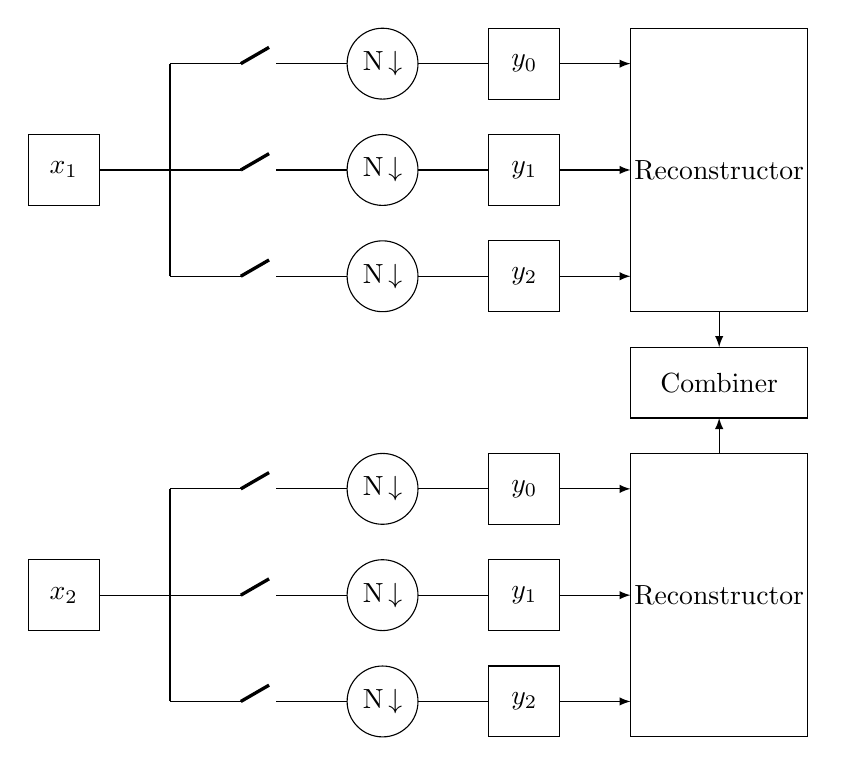
\begin{tikzpicture}[scale=.9]
\draw  (-2.5,2) rectangle (-1.5,1) node[pos=.5]{$x_1$};
\draw  (-1.5,1.5) -- (0.5,1.5);
\draw  (-0.5,3) -- (0.5,3);
\draw (-0.5,3) --(-.5,0) ;

\draw (-0.5,0) -- (0.5,0);

\draw  (1,3) -- (2,3);
\draw  (1,1.5) -- (2,1.5);
\draw  (1,0) -- (2,0);

\draw[ very thick](0.5,3)-- +(30:0.46);
\draw[ very thick](0.5,1.5)-- +(30:0.46);
\draw[ very thick](0.5,0)-- +(30:0.46);

\draw  (2.5,3) ellipse (.5 and .5) node{N$\,\downarrow$} ;
\draw  (2.5,1.5) ellipse (.5 and .5) node{N$\,\downarrow$} ;
\draw  (2.5,0) ellipse (.5 and .5) node{N$\,\downarrow$} ;

\draw  [>=latex,->] (5,3) -- (6,3);
\draw  [>=latex,->] (5,1.5) -- (6,1.5);
\draw  [>=latex,->] (5,0) -- (6,0);

\draw  (3,3) -- (4,3);
\draw  (3,1.5) -- (4,1.5);
\draw  (3,0) -- (4,0);

\draw  (5,3.5) rectangle (4,2.5) node[pos=.5]{$y_0$};
\draw  (5,2) rectangle (4,1) node[pos=.5]{$y_1$};
\draw  (5,0.5) rectangle (4,-0.5) node[pos=.5]{$y_2$};

\draw  (-2.5,-4) rectangle (-1.5,-5) node[pos=.5]{$x_2$};
\draw  (-1.5,-4.5) -- (0.5,-4.5);
\draw  (-0.5,-3) -- (0.5,-3);
\draw (-0.5,-3) --(-0.5,-6) ;

\draw (-0.5,-6) -- (0.5,-6);

\draw  (1,-3) -- (2,-3);
\draw  (1,-4.5) -- (2,-4.5);
\draw  (1,-6) -- (2,-6);

\draw[ very thick](0.5,-3)-- +(30:0.46);
\draw[ very thick](0.5,-4.5)-- +(30:0.46);
\draw[ very thick](0.5,-6)-- +(30:0.46);

\draw  (2.5,-3) ellipse (.5 and .5) node{N$\,\downarrow$} ;
\draw  (2.5,-4.5) ellipse (.5 and .5) node{N$\,\downarrow$} ;
\draw  (2.5,-6) ellipse (.5 and .5) node{N$\,\downarrow$} ;

\draw  (3,-3) -- (4,-3);
\draw  (3,-4.5) -- (4,-4.5);
\draw  (3,-6) -- (4,-6);

\draw  [>=latex,->] (5,-3) -- (6,-3);
\draw  [>=latex,->] (5,-4.5) -- (6,-4.5);
\draw  [>=latex,->] (5,-6) -- (6,-6);

\draw  (5,-2.5) rectangle (4,-3.5) node[pos=.5]{$y_0$};
\draw  (5,-4) rectangle (4,-5) node[pos=.5]{$y_1$};
\draw  (5,-5.5) rectangle (4,-6.5) node[pos=.5]{$y_2$};

\draw  (6,3.5) rectangle (8.5,-.5) node[pos=.5]{Reconstructor};
\draw  (6,-2.5) rectangle (8.5,-6.5) node[pos=.5]{Reconstructor};

\draw  (6,-1) rectangle (8.5,-2) node[pos=.5]{Combiner};
\draw [>=latex,->] (7.25,-2.5) -- (7.25,-2);
\draw [>=latex,->] (7.25,-.5) -- (7.25,-1);

\end{tikzpicture}
\caption{Schematic of collaborative sampling implementation}\label{tkz:sc_collaborative}
\end{figure}


\subsection{Coprime sampling}\label{sub:coprime}
Coprime sampling is different from circular sparse sampling and collaborative sampling in the sense that the different sampler sample with differents periods. Also, the amount of samplers is restricted to two. The first sampler samples with period $aT$, and the second sampler samples with period $bT$. Coprime sampling is illustrated in \cref{tkz:coprime}. In this example, $a=3$ and $b=5$.

\begin{figure}[H]
\centering
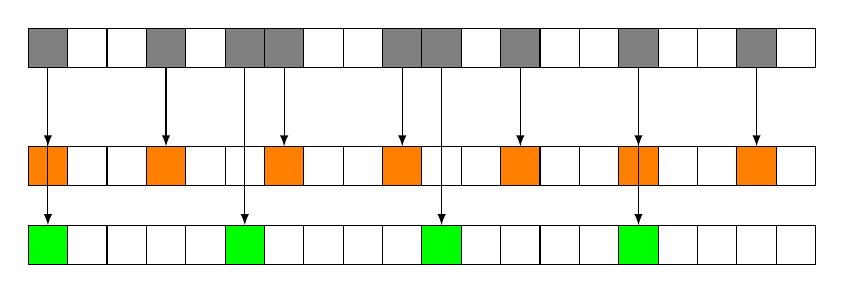
\begin{tikzpicture}
\draw  [fill=gray](-1,0.5) rectangle (-0.5,0);
\draw  (-0.5,0.5) rectangle (0,0);
\draw  (0,0.5) rectangle (0.5,0);
\draw  [fill=gray](0.5,0.5) rectangle (1,0);
\draw  (1,0.5) rectangle (1.5,0);
\draw  [fill=gray](1.5,0.5) rectangle (2,0);
\draw  [fill=gray](2,0.5) rectangle (2.5,0);
\draw  (2.5,0.5) rectangle (3,0);
\draw  (3,0.5) rectangle (3.5,0);
\draw  [fill=gray](3.5,0.5) rectangle (4,0);
\draw [fill=gray] (4,0.5) rectangle (4.5,0);
\draw  (4.5,0.5) rectangle (5,0);
\draw  [fill=gray](5,0.5) rectangle (5.5,0);
\draw  (5.5,0.5) rectangle (6,0);
\draw  (6,0.5) rectangle (6.5,0);
\draw [fill=gray](6.5,0.5) rectangle (7,0);
\draw  (7,0.5) rectangle (7.5,0);
\draw  (7.5,0.5) rectangle (8,0);
\draw  [fill=gray](8,0.5) rectangle (8.5,0);
\draw  (8.5,0.5) rectangle (9,0);

\draw  [fill=orange](-1,-1) rectangle (-0.5,-1.5);
\draw  (-0.5,-1) rectangle (0,-1.5);
\draw  (0,-1) rectangle (0.5,-1.5);
\draw  [fill=orange](0.5,-1) rectangle (1,-1.5);
\draw  (1,-1) rectangle (1.5,-1.5);
\draw  (1.5,-1) rectangle (2,-1.5);
\draw  [fill=orange](2,-1) rectangle (2.5,-1.5);
\draw  (2.5,-1) rectangle (3,-1.5);
\draw  (3,-1) rectangle (3.5,-1.5);
\draw  [fill=orange](3.5,-1) rectangle (4,-1.5);
\draw  (4,-1) rectangle (4.5,-1.5);
\draw  (4.5,-1) rectangle (5,-1.5);
\draw  [fill=orange](5,-1) rectangle (5.5,-1.5);
\draw  (5.5,-1) rectangle (6,-1.5);
\draw  (6,-1) rectangle (6.5,-1.5);
\draw  [fill=orange](6.5,-1) rectangle (7,-1.5);
\draw  (7,-1) rectangle (7.5,-1.5);
\draw  (7.5,-1) rectangle (8,-1.5);
\draw  [fill=orange](8,-1) rectangle (8.5,-1.5);
\draw  (8.5,-1) rectangle (9,-1.5);

\draw  [fill=green](-1,-2) rectangle (-0.5,-2.5);
\draw  (-0.5,-2) rectangle (0,-2.5);
\draw  (0,-2) rectangle (0.5,-2.5);
\draw  (0.5,-2) rectangle (1,-2.5);
\draw  (1,-2) rectangle (1.5,-2.5);
\draw [fill=green] (1.5,-2) rectangle (2,-2.5);
\draw  (2,-2) rectangle (2.5,-2.5);
\draw  (2.5,-2) rectangle (3,-2.5);
\draw  (3,-2) rectangle (3.5,-2.5);
\draw  (3.5,-2) rectangle (4,-2.5);
\draw  [fill=green](4,-2) rectangle (4.5,-2.5);
\draw  (4.5,-2) rectangle (5,-2.5);
\draw  (5,-2) rectangle (5.5,-2.5);
\draw  (5.5,-2) rectangle (6,-2.5);
\draw  (6,-2) rectangle (6.5,-2.5);
\draw [fill=green] (6.5,-2) rectangle (7,-2.5);
\draw  (7,-2) rectangle (7.5,-2.5);
\draw  (7.5,-2) rectangle (8,-2.5);
\draw  (8,-2) rectangle (8.5,-2.5);
\draw  (8.5,-2) rectangle (9,-2.5);

\draw [>=latex,->] (-.75,0) to (-.75,-1);
\draw [>=latex,->] (.75,0) to (.75,-1);
\draw [>=latex,->] (2.25,0) to (2.25,-1);
\draw [>=latex,->] (3.75,0) to (3.75,-1);
\draw [>=latex,->] (5.25,0) to (5.25,-1);
\draw [>=latex,->] (6.75,0) to (6.75,-1);
\draw [>=latex,->] (8.25,0) to (8.25,-1);

\draw [>=latex,->] (-.75,0) to (-.75,-2);
\draw [>=latex,->] (1.75,0) to (1.75,-2);
\draw [>=latex,->] (4.25,0) to (4.25,-2);
\draw [>=latex,->] (6.75,0) to (6.75,-2);

\end{tikzpicture}
\caption{Coprime sampling with $a=3$ and $b=5$}\label{tkz:coprime}
\end{figure}
The choice of the $a$ and $b$ substantially influences the performance of the coprime sampler. This influence will be investigated in \cref{sec:coprime}. 

In \cref{sec:reconstruction-algorithm}, it is assumed that every sampler samples the input signal at a same rate. However, coprime sampling involves two samplers sampling at different rates. Therefore, using the reconstruction algorithm in conjunction with coprime sampling is non-trivial. \Cref{tkz:sc_coprime} shows an equivalent hardware implementation, which may be used for reconstruction. This implementation will be further discussed in \cref{sec:coprime}. It is worthwhile to note that the equivalent signals $u_0,\ldots,u_a$ and $v_0,\ldots,v_b$ are an $a\cdot b$-decimation of the input signal.

\begin{figure}[H]
\centering
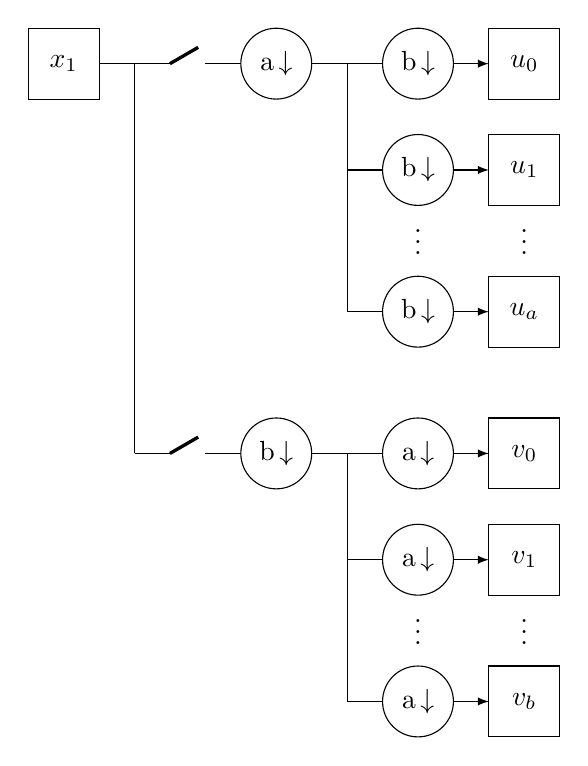
\begin{tikzpicture}[scale=.9]

\draw  (-2.5,3.5) rectangle (-1.5,2.5) node[pos=.5]{$x_1$};

\draw  (-1.5,3) -- (-0.5,3);
\draw  (0,3) -- (0.5,3);
\draw  (2,1.5) -- (2.5,1.5);
\draw  (2,-0.5) -- (2.5,-0.5);

\draw[ very thick](-0.5,3)-- +(30:0.46);

\draw  (1,3) ellipse (.5 and .5) node{a$\,\downarrow$} ;
\draw  (3,3) ellipse (.5 and .5) node{b$\,\downarrow$} ;
\draw  (3,1.5) ellipse (.5 and .5) node{b$\,\downarrow$} ;
\draw  (3,-0.5) ellipse (.5 and .5) node{b$\,\downarrow$} ;

\node at (4.5,0.6) {\vdots};
\node at (3,0.6) {\vdots};

\draw  (1.5,3) -- (2.5,3);

\draw [>=latex,->] (3.5,3) -- (4,3);
\draw [>=latex,->] (3.5,1.5) -- (4,1.5);
\draw [>=latex,->] (3.5,-0.5) -- (4,-0.5);

\draw  (2,-0.5) -- (2,3);

\draw  (5,3.5) rectangle (4,2.5) node[pos=.5]{$u_0$};
\draw  (5,2) rectangle (4,1) node[pos=.5]{$u_1$};
\draw  (5,0) rectangle (4,-1) node[pos=.5]{$u_a$};

%%%%%%%%%%%%%%%

\draw  (-1,-2.5) -- (-1,3);
\draw  (-1,-2.5) -- (-0.5,-2.5);

\draw  (0,-2.5) -- (0.5,-2.5);
\draw  (2,-4) -- (2.5,-4);
\draw  (2,-6) -- (2.5,-6);

\draw[ very thick](-0.5,-2.5)-- +(30:0.46);

\draw  (1,-2.5) ellipse (.5 and .5) node{b$\,\downarrow$} ;
\draw  (3,-2.5) ellipse (.5 and .5) node{a$\,\downarrow$} ;
\draw  (3,-4) ellipse (.5 and .5) node{a$\,\downarrow$} ;
\draw  (3,-6) ellipse (.5 and .5) node{a$\,\downarrow$} ;

\node at (4.5,-4.9) {\vdots};
\node at (3,-4.9) {\vdots};

\draw  (1.5,-2.5) -- (2.5,-2.5);

\draw [>=latex,->] (3.5,-2.5) -- (4,-2.5);
\draw [>=latex,->] (3.5,-4) -- (4,-4);
\draw [>=latex,->] (3.5,-6) -- (4,-6);

\draw  (2,-6) -- (2,-2.5);

\draw  (5,-2) rectangle (4,-3) node[pos=.5]{$v_0$};
\draw  (5,-3.5) rectangle (4,-4.5) node[pos=.5]{$v_1$};
\draw  (5,-5.5) rectangle (4,-6.5) node[pos=.5]{$v_b$};

\end{tikzpicture}
\caption{Schematic of an equivalent hardware implementation of coprime sampling}\label{tkz:sc_coprime}
\end{figure}
\end{document}

